% =====================================================================
%  Project-I Review-2 Report
%  Trust-Aware Continual Learning for IoT Intrusion Detection
%
%  Compile on Overleaf with pdfLaTeX. Two passes for the ToC/refs.
%  Self-contained: every figure is drawn in TikZ/pgfplots, so there are
%  no external image files to upload.
%
%  >>> FILL IN THE PLACEHOLDERS MARKED  %% TODO  ON THE TITLE PAGE. <<<
% =====================================================================
\documentclass[12pt,a4paper]{report}

\usepackage[a4paper,left=1.25in,right=1in,top=1in,bottom=1in]{geometry}
\usepackage{mathptmx}                 % Times text + math
\usepackage[T1]{fontenc}
\usepackage[utf8]{inputenc}
\usepackage{amsmath,amssymb}
\usepackage{graphicx}
\usepackage{booktabs}
\usepackage{array}
\usepackage{longtable}
\usepackage{caption}
\usepackage{enumitem}
\usepackage{xcolor}
\usepackage{tikz}
\usepackage{pgfplots}
\pgfplotsset{compat=1.18}
\usetikzlibrary{positioning,arrows.meta,shapes.geometric,fit,calc,backgrounds}
\usepackage[hidelinks]{hyperref}
\usepackage{setspace}

\onehalfspacing
\setlength{\parindent}{0.5in}
\captionsetup[table]{skip=4pt,font=small,labelfont=bf}
\captionsetup[figure]{skip=6pt,font=small,labelfont=bf}
\renewcommand{\arraystretch}{1.25}

% chapter headings that read like the template's numbered sections
\usepackage{titlesec}
\titleformat{\chapter}[hang]{\normalfont\large\bfseries\filcenter}
  {\thechapter.}{1em}{\MakeUppercase}
\titlespacing*{\chapter}{0pt}{0pt}{20pt}
\titleformat{\section}[hang]{\normalfont\normalsize\bfseries}{\thesection}{1em}{}
\titleformat{\subsection}[hang]{\normalfont\normalsize\bfseries\itshape}{\thesubsection}{1em}{}

\newcommand{\note}[1]{\par\medskip{\small\itshape #1}\par\medskip}

% colours shared by the diagrams
\definecolor{cGrey}{HTML}{6B7280}
\definecolor{cBlue}{HTML}{1E5F9E}
\definecolor{cBlueF}{HTML}{EAF2FB}
\definecolor{cTeal}{HTML}{0F766E}
\definecolor{cTealF}{HTML}{E6F4F1}
\definecolor{cAmber}{HTML}{B45309}
\definecolor{cAmberF}{HTML}{FDF3E3}
\definecolor{cPurple}{HTML}{7C3AED}
\definecolor{cPurpleF}{HTML}{F5F0FE}
\definecolor{cRed}{HTML}{8B1A1A}
\definecolor{cGreen}{HTML}{2CA02C}
\definecolor{cOrange}{HTML}{FF7F0E}

\begin{document}

% =====================================================================
\begin{titlepage}
\centering
{\large\bfseries BCSE497J - Project-I\par}   %% TODO confirm course code
\vspace{1.4cm}
{\Large\bfseries Trust-Aware Continual Learning for IoT\\[2pt]
Intrusion Detection: An Evidence-Based\\[2pt]
Authorization Gate Against Slow Poisoning\par}
\vspace{1.4cm}
{\normalsize
\begin{tabular}{ll}
\textbf{<<REG NO>>} & \textbf{<<STUDENT NAME>>}\\   %% TODO
\textbf{<<REG NO>>} & \textbf{<<STUDENT NAME>>}\\   %% TODO
\end{tabular}\par}
\vspace{1.2cm}
{\normalsize Under the Supervision of\par}
\vspace{0.5cm}
{\normalsize\bfseries <<GUIDE NAME>>\par}          %% TODO
{\normalsize\bfseries <<DESIGNATION>>\par}         %% TODO
{\normalsize School of Computer Science and Engineering (SCOPE)\par}
\vspace{1.6cm}
{\normalsize\bfseries B.Tech.\par}
{\normalsize\itshape in\par}
{\normalsize\bfseries Computer Science and Engineering\par}
\vspace{0.4cm}
{\normalsize\bfseries School of Computer Science and Engineering\par}
\vspace{1.6cm}
{\normalsize Vellore Institute of Technology\par}
\vspace{0.8cm}
{\normalsize September 2026\par}
\end{titlepage}

\pagenumbering{arabic}
\setcounter{page}{1}

% =====================================================================
\chapter*{Abstract}
\addcontentsline{toc}{chapter}{Abstract}
\setcounter{chapter}{0}

An intrusion detection system that continues to learn after deployment can be
taught the wrong thing. Adaptation is necessary because real networks change,
but an adversary who knows the detector adapts can pace malicious traffic so
that its statistical signature migrates slowly toward the benign region, until
the detector has been taught that the attack is normal. Existing defences judge
a proposed update by inspecting the training data itself; a patient attacker
controls that data, and therefore controls the evidence.

This project builds and evaluates an \emph{authorization gate} placed between
drift detection and model update in an online intrusion detection system. The
gate combines three traffic-derived evidence signals -- attribution consistency,
topology diversity and temporal stability -- into a trust score, and then
cross-checks that score against an out-of-band reputation channel that is not a
function of the traffic. The reputation channel may veto an update regardless of
how healthy the traffic evidence appears. Four arms run through one common
orchestrator on identical data: a frozen detector that never updates, an ungated
detector that accepts every proposal, a traffic-only gate representing existing
evidence-based gating, and the proposed gate.

Evaluated on real N-BaIoT traffic (Danmini\_Doorbell; 115 features; 49{,}548
benign and 107{,}685 Mirai records, verified free of missing and infinite
values), a slow-poisoning campaign defeated the traffic-only gate: it accepted
five poisoned updates and its detection of a subsequent full-strength repeat of
the attack it had been calibrated on fell to 0.200. The proposed gate refused
all twenty-four proposals and retained detection of 1.000. At round 40 both
gates observed numerically identical evidence ($A{=}0.500$, $P{=}0.784$,
$S{=}0.459$, $T{=}0.573$) and reached opposite decisions; only the independent
channel separated them. A second finding emerged from the traces: having
accepted one poisoned update, the traffic-only gate's own reference frame moved,
inflating its attribution score on later poisoned windows from 0.500 to as high
as 0.956, so that accepting one unauthorized update made accepting the next more
likely.

Two negative results are reported rather than withheld. The genuine-drift
scenario produced no adaptation at all: a benign-to-benign device shift of
5.7 standard deviations never crossed the decision boundary, the frozen detector
continued to score 0.998, and the error-driven change detector therefore never
fired. And the out-of-band signal is simulated from ground-truth traffic origin,
because the dataset carries no reputation field; the defensible claim is
therefore what an authorization step achieves \emph{once an independent signal
exists}, not that this work detects the attacker.

\vspace{0.6cm}
\noindent\textbf{Keywords} -- intrusion detection; continual learning; concept
drift; data poisoning; adversarial machine learning; authorization; runtime
assurance; out-of-band verification; N-BaIoT; prequential evaluation; negative
results; reproducibility.

% =====================================================================
\newpage
\tableofcontents
\newpage

% =====================================================================
\chapter{Introduction}

\section{Background}

Network intrusion detection systems are trained on traffic captured at one
moment and deployed into networks that do not stay still. Devices receive
firmware updates, usage patterns change with the season and the working day, and
new services appear. A detector whose decision boundary is fixed at training
time drifts out of alignment with the traffic it inspects, and the practical
symptom is a rising false alarm rate that erodes operator trust until the system
is ignored or switched off.

The established response is continual, or online, learning: the detector keeps
consuming traffic after deployment and periodically revises what it considers
normal. Streaming learners of this kind, paired with a change detector that
signals when the distribution has moved, are well developed. The assumption
underlying them is that the change being adapted to is genuine -- that the world
moved, and the model should follow.

That assumption is a security property, and it is not free. An adversary who
knows the detector adapts is presented with an additional attack surface that a
frozen detector does not have. Rather than attempting to evade the current
decision boundary, the adversary can attempt to move it. If malicious traffic is
introduced gradually enough, each individual increment is small enough to look
like ordinary drift, and the detector may be persuaded to absorb the attack into
its own notion of normal behaviour. This is a causative, or training-time,
attack, and it is qualitatively different from evasion because its damage
persists after the attack traffic stops.

\section{Motivation}

Two observations motivate this project.

First, the decision to accept a model update is currently implicit. In a typical
adaptive pipeline, a change detector fires and the model retrains; nothing sits
between the two. There is no point in the architecture at which the question
``should this update be permitted?'' is asked as a separate, answerable
question, and consequently no place where an answer could be recorded, audited,
or refused.

Second, and more fundamentally, the defences that do exist judge a proposed
update using evidence extracted from the data being learned from. Trimmed-loss
defences inspect the training set; drift detectors watch an error stream that
the poisoned data itself produces; regularisation methods anchor against a
signal derived from the same source. Each of these is a measurement of a channel
the attacker is actively shaping. A sufficiently patient adversary can satisfy
all of them simultaneously, not by defeating any particular statistic, but by
being willing to move slowly.

This project therefore treats the authorization decision itself as the object of
study. It asks whether a gate that consults a signal originating outside the
traffic channel can refuse an update that traffic-derived evidence alone would
approve, and it measures the consequences of getting that decision wrong.

\section{Scope of the Project}

The project delivers a complete streaming intrusion detection pipeline with an
explicit authorization stage, a four-arm controlled comparison run through a
single orchestrator, an evaluation on real N-BaIoT traffic, and an interactive
demonstration front end that replays the decision sequence.

The boundaries are stated here and reported as results rather than concealed.

\begin{itemize}[leftmargin=*,itemsep=3pt]
\item \textbf{The out-of-band signal is simulated.} N-BaIoT contains no
destination address, no reputation field and no command-and-control cost
indicator. The reputation channel is therefore keyed to ground-truth traffic
origin. It is not derived from the feature vector, which preserves its
independence in principle, but it is closer to an oracle than a deployed
threat-intelligence feed would be.
\item \textbf{The attacker's pacing is constructed.} Real N-BaIoT capture files
are not temporally paced to be slow. The poisoning schedule is imposed by
interpolating between real attack records and real benign records; every
endpoint is genuine captured traffic, but the schedule is ours.
\item \textbf{One device family, one attack family.} The primary evaluation uses
Danmini\_Doorbell with the Mirai \texttt{scan} attack, plus Ennio\_Doorbell
benign traffic as a second operating point.
\item \textbf{No hyper-parameter tuning.} Thresholds and evidence weights are
untuned defaults chosen before any result was seen.
\item \textbf{No automated test suite.} The project relies on scripted
verification of specific claims rather than on unit tests. This is a genuine
deficiency and is recorded as such in Section~4.3.
\item \textbf{No claim of mechanism novelty in drift detection or online
learning.} The change detector and the streaming classifier are existing,
standard components used as published.
\end{itemize}

% =====================================================================
\chapter{Project Description and Goals}

\section{Literature Review}

The relevant literature falls into three groups: the machinery of adaptation
under concept drift, the adversarial manipulation of learners that adapt, and
the defences proposed against it. Table~\ref{tab:lit} records the works relied
upon and the specific contribution taken from each.

\begin{table}[htbp]
\centering
\caption{Literature relied upon and the contribution taken from each.}
\label{tab:lit}
\small
\begin{tabular}{@{}p{0.5cm}p{4.2cm}p{8.0cm}@{}}
\toprule
\textbf{Ref} & \textbf{Work} & \textbf{Contribution relied upon}\\
\midrule
[1] & Sommer \& Paxson, IEEE S\&P 2010 &
Why machine learning underperforms specifically for intrusion detection; the
evaluation traps this report is written to avoid\\
[2] & Gama et al., ACM Computing Surveys 2014 &
Vocabulary and taxonomy for concept drift and its adaptation; establishes that
the adversarial case sits outside the standard framing\\
[3] & Bifet \& Gavald\`a, SDM 2007 &
ADWIN: adaptive windowing over an error stream, used unmodified as this
project's change detector\\
[4] & Montiel et al., JMLR 2021 &
The River streaming-learning library; incremental estimators and prequential
metrics used for all four arms\\
[5] & Meidan et al., IEEE Pervasive Computing 2018 &
The N-BaIoT dataset and its 115-feature streaming representation; also the
source of the absent reputation field\\
[6] & Barreno et al., ASIACCS 2006 &
The causative versus exploratory attack distinction that names this project's
threat model\\
[7] & Nelson et al., USENIX LEET 2008 &
Poisoning of a deployed, continually retraining classifier; the closest prior
threat to the one studied here\\
[8] & Biggio et al., ICML 2012 &
The canonical optimisation-based poisoning attack against a batch learner\\
[9] & Jagielski et al., IEEE S\&P 2018 &
Poisoning attacks together with the TRIM defence; the closest defence baseline,
and one that inspects only the training data\\
[10] & Kirkpatrick et al., PNAS 2017 &
Elastic Weight Consolidation; limits forgetting but cannot refuse an update, a
distinction this project depends on\\
[11] & Arp et al., USENIX Security 2022 &
Methodological pitfalls in machine learning for security; the checklist against
which this report's disclosures are written\\
\bottomrule
\end{tabular}
\end{table}

\note{Verification status. The works above are cited from standard knowledge of
the field. Titles, authors, venues and years are believed correct; exact volume,
issue and page numbers should be confirmed against the primary sources before
final submission, and Section~5 marks the entries most likely to need
correction. No claim in this report depends on an unverified reference for its
substance.}

\section{Research Gap}

The gap addressed here is one of architecture rather than of statistics. Three
specific deficiencies were identified.

\textbf{No explicit authorization stage.} In the standard adaptive pipeline a
detected change point leads directly to a model update. The decision to accept
that update is never represented as a decision, and so cannot be constrained,
recorded or refused.

\textbf{Defences confined to the attacker's own channel.} Every defence surveyed
judges a proposed update by inspecting the data the update is derived from.
TRIM~[9] trims the training set. EWC~[10] anchors weights against the training
signal. Drift detectors~[3] watch an error stream that the poisoned data itself
produces. Each is a measurement of a quantity the adversary is shaping, so a
patient adversary can satisfy all of them at once.

\textbf{Damage measured only while the attack is in progress.} Poisoning is
usually scored by accuracy during the attack window. The more consequential
question -- whether the detector can still recognise an unmistakable instance of
the original attack \emph{afterwards} -- is asked far less often, and it is the
question that distinguishes a temporary evasion from durable corruption.

\note{What this project does not claim. The streaming classifier, the change
detector and the poisoning strategy are all existing techniques used as
published. The contribution is the interposition of an authorization decision
whose deciding input is not a function of the traffic being judged, together
with an honest measurement of what happens when that decision is delegated to
traffic-derived evidence alone.}

\section{Objectives}

Table~\ref{tab:obj} states each objective with the criterion by which it was
judged and its outcome. Objectives O1--O6 concern the mechanism and its
evaluation; O7 and O8 concern reproducibility and demonstration. Two objectives
are recorded as \emph{not achieved}, and the reasons are given in
Section~4.3.

\begin{table}[htbp]
\centering
\caption{Project objectives and their completion status.}
\label{tab:obj}
\small
\begin{tabular}{@{}p{0.7cm}p{3.9cm}p{4.2cm}p{4.0cm}@{}}
\toprule
\textbf{\#} & \textbf{Objective} & \textbf{Measurable criterion} & \textbf{Outcome}\\
\midrule
O1 & Build a prequential online IDS with change detection on real IoT traffic &
Predict-then-train enforced for every record; no label seen before prediction &
Achieved -- 115-feature N-BaIoT stream, 80 rounds\\
O2 & Define traffic-derived trust evidence and quantify its limits &
Three signals in $[0,1]$; adversary's ability to shape each stated &
Achieved -- $A$, $P$, $S$; all three shown shapeable\\
O3 & Establish that the evidence layer is numerically sound on real data &
Evidence must not be dominated by feature scale &
Achieved -- defect found and corrected; see Section~4.3.1\\
O4 & Interpose an authorization gate with an independent veto &
Veto must be able to refuse an update the evidence approves &
Achieved -- 5 such refusals, rounds 40 and 72--75\\
O5 & Compare four arms through one orchestrator under slow poisoning &
Identical data, identical trigger, one method differing per arm &
Achieved -- 4 arms, 80 rounds, real traffic\\
O6 & Measure durable damage, not only damage during the attack &
Detection of a full-strength repeat of the calibrated attack &
Achieved -- 0.200 versus 1.000\\
O7 & Demonstrate that the gate does not obstruct legitimate drift &
Genuine benign drift should be authorized, not refused &
\textbf{Not achieved} -- no drift was triggered; see Section~4.3.5\\
O8 & Make the pipeline reproducible and demonstrable &
Deterministic re-run; interactive replay of every decision &
Partially achieved -- replay delivered; no automated test suite\\
\bottomrule
\end{tabular}
\end{table}

\section{Problem Statement}

Given an intrusion detection system that continues to learn from live traffic,
and an adversary who is aware of that fact and is willing to act slowly,
interpose a deterministic authorization stage between change detection and model
update, and answer two questions with measurement rather than assertion.

First: can traffic-derived evidence alone distinguish a legitimate adaptation
from a paced poisoning campaign? Second: if it cannot, does a signal that is not
a function of the traffic recover the distinction, and what is the measurable
cost of having got that decision wrong once the attack has ended?

\section{Project Plan}

Figure~\ref{fig:plan} records the work in the order it was carried out. The
repository's version-control history begins on 7 September 2026, the date the
repository was initialised; the earlier development predates that and the
chronology below is reconstructed from the dated artefacts rather than from
commit timestamps. This is stated because commit dates alone would misrepresent
the schedule.

\begin{figure}[htbp]
\centering
\begin{tikzpicture}[x=1.05cm,y=0.62cm,font=\scriptsize]
\def\tasks{
  {Pipeline on synthetic stream, four arms}/0/3.0/cBlue,
  {Real N-BaIoT acquisition and integrity checks}/3.0/1.6/cBlue,
  {Feature-scale defect found and corrected}/4.6/1.4/cRed,
  {Real-data stream builders, paced poisoning}/6.0/1.8/cTeal,
  {Slow-poisoning campaign, 80 rounds}/7.8/1.4/cTeal,
  {Second device acquired; drift scenario}/9.2/1.4/cAmber,
  {Interactive replay front end}/10.6/2.0/cPurple,
  {Diagrams, report, Review-2 preparation}/12.6/2.4/cGrey
}
\foreach \name/\start/\len/\col [count=\i] in \tasks {
  \node[anchor=east,align=right,text width=5.4cm] at (0,-\i) {\name};
  \fill[\col,rounded corners=1pt] (\start*0.85+0.25,-\i-0.22)
        rectangle (\start*0.85+\len*0.85+0.25,-\i+0.22);
}
\draw[cGrey,-{Stealth[length=4pt]}] (0.25,-8.9) -- (13.6,-8.9);
\foreach \x/\lab in {0.25/{start},3.05/{},6.15/{},9.1/{},12.0/{Review 2}}
  \draw[cGrey] (\x,-8.75) -- (\x,-9.05) node[below,font=\tiny] {\lab};
\draw[cRed,dashed] (12.0,-0.4) -- (12.0,-9.1);
\end{tikzpicture}
\caption{Project plan -- execution chronology, reconstructed from dated
artefacts. The red rule marks Review 2.}
\label{fig:plan}
\end{figure}

% =====================================================================
\chapter{Technical Specification}

\section{Requirements}

The requirements below were derived from the implemented system; each
corresponds to a module that exists in the repository.

\subsection{Functional}

\textbf{Stream ingestion.} The system shall present network records as a stream
of \texttt{(features, label, metadata)} tuples, with an identical interface for
the synthetic and the real N-BaIoT source, so that no downstream component
depends on which is in use.

\textbf{Prequential evaluation.} The system shall, for every record, predict
before training on that record, and shall never expose a label to the model
before its prediction has been scored.

\textbf{Change detection.} The system shall monitor the error stream of the
frozen arm and open a bounded adaptation window when a change point is
signalled. Outside that window no update shall be proposed to any arm.

\textbf{Evidence extraction.} The system shall compute three traffic-derived
signals in $[0,1]$ from the window under consideration, in a feature space
calibrated on trusted data and thereafter frozen.

\textbf{Authorization.} The system shall decide, for each proposed update,
whether to accept it, and shall record the decision together with the reason.

\textbf{Independent veto.} The system shall consult a reputation signal that is
not derived from the feature vector, and shall permit that signal to refuse an
update irrespective of the traffic evidence.

\textbf{Null effect of refusal.} A refused update shall alter nothing: neither
the model, nor the trusted baseline, nor the reference drift direction.

\textbf{Controlled comparison.} The system shall run four arms over identical
data with an identical change trigger, differing in exactly one respect each.

\textbf{Decision logging.} The system shall persist, per round and per arm,
every evidence value, the trust score, the reputation, the decision, the stated
reason and both windowed and cumulative accuracy.

\textbf{Replay.} The system shall replay a recorded run one round at a time,
exposing classification, evidence and the authorization decision as they
occurred.

\subsection{Non-Functional}

\textbf{Determinism.} Given the same inputs, a re-run shall reproduce the same
decisions; all sampling is seeded.

\textbf{Trust boundary integrity.} The evidence feature space shall be fitted on
calibration data only and never refitted on live windows, so that the reference
frame cannot be moved by an adversary.

\textbf{Trigger independence.} The change detector shall observe an arm that
never updates, so that no arm's own decisions can corrupt the trigger for the
others.

\textbf{Auditability.} Every authorization decision shall be explainable from
stored records without re-running the pipeline.

\textbf{Portability.} The system shall run on commodity hardware with no
discrete graphics processor and no cloud service.

\textbf{Numerical soundness.} Geometric evidence shall be computed only in a
space where features contribute on comparable scales.

\section{Feasibility Study}

\subsection{Technical Feasibility}

Technical feasibility is demonstrated rather than argued: the system is
implemented and runs end to end on real data. The complete four-arm campaign
over 80 rounds of 115-feature N-BaIoT traffic completes in under two minutes on
the machine in Table~\ref{tab:hw}, with no discrete graphics processor and no
network access once the dataset is local. The streaming classifier is linear and
the evidence layer is a handful of vector operations per round, so the cost is
dominated by reading the capture files.

\subsection{Economic Feasibility}

The project incurs no licensing or infrastructure cost. Python, River, NumPy,
pandas, Streamlit and Altair are open source; the N-BaIoT dataset is publicly
archived and free to download. No cloud compute, paid interface subscription or
specialised hardware is required.

\note{No costing study, budget projection or return-on-investment analysis was
performed, and none is claimed. Statements about deployment economics would
require operational data this project does not have.}

\subsection{Social Feasibility}

An intrusion detector that can be silently taught to ignore an attack is a
safety problem for everyone downstream of it, and the mechanism studied here is
intended to make that failure mode visible and refusable rather than silent.
Every authorization decision is recorded with its reason, which is a
precondition for an operator to audit why a detector did or did not adapt.

\note{No user study, operator interview or human-subjects work was conducted.
The reputation channel is simulated, so no claim is made about the behaviour of
a real threat-intelligence feed or about its own failure modes, which in
deployment would include both false accusation and stale intelligence.}

\section{System Specification}

\subsection{Hardware Specification}

\begin{table}[htbp]
\centering
\caption{Hardware specification -- the development and evaluation platform.}
\label{tab:hw}
\small
\begin{tabular}{@{}p{3.6cm}p{9.6cm}@{}}
\toprule
\textbf{Component} & \textbf{Specification}\\
\midrule
Processor & 12th Generation Intel Core i5-12500H; 12 physical cores, 16 logical\\
Memory & 15.7 GB\\
Graphics & NVIDIA GeForce RTX 3050 Laptop GPU present but unused; all
computation is CPU-bound\\
Operating system & Windows 11 Home Single Language, build 10.0.26200, 64-bit\\
Storage & Local solid-state storage; approximately 285 MB of capture files\\
Network & Required only to download the dataset; all experiments run offline\\
\bottomrule
\end{tabular}
\end{table}

\subsection{Software Specification}

\begin{table}[htbp]
\centering
\caption{Software specification, with the versions actually used.}
\label{tab:sw}
\small
\begin{tabular}{@{}p{3.6cm}p{9.6cm}@{}}
\toprule
\textbf{Category} & \textbf{Software}\\
\midrule
Language & Python 3.13.7\\
Streaming ML & River 0.26.1 -- \texttt{StandardScaler}, \texttt{LogisticRegression},
\texttt{ADWIN}, prequential \texttt{Accuracy} and \texttt{F1}\\
Numerics & NumPy 2.5.3; pandas 3.0.5; SciPy 1.18.1\\
Front end & Streamlit 1.63.0 with Altair for interactive charts\\
Plotting & Matplotlib 3.11.1 for static figures\\
Version control & Git; repository hosted on GitHub\\
\bottomrule
\end{tabular}
\end{table}

% =====================================================================
\chapter{Design Approach and Details}

\section{System Architecture}

The system is a streaming detection pipeline organised in three tiers with
exactly one route from a proposed update to the model. Figure~\ref{fig:arch}
shows the arrangement.

The \textbf{adaptation tier} is the proposer. When the change detector signals
that the distribution has moved, this tier proposes that the current window be
treated as normal -- that is, it relabels the window and offers it to the model
as training data. It is untrusted by construction: every signal that can be
computed about the window is computed from traffic the adversary may be shaping.

The \textbf{authorization tier} is the gate. It runs on every proposed update,
combines the three evidence signals into a trust score $T$, and cross-checks $T$
against the out-of-band reputation $R$. It is the sole route from a proposal to
the model. Its deciding advantage over the tier above it is not a better
statistic but a different \emph{source}: $R$ is not a function of the feature
vector, so shaping the traffic does not move it.

The \textbf{model tier} is the online detector itself: a standardiser feeding a
logistic regression, evaluated prequentially.

Two components sit deliberately outside the update path. The reputation channel
enters the gate from the side and is never derived from the window. The decision
log receives a copy of every decision and returns nothing, so it cannot
influence what the model learns.

\begin{figure}[htbp]
\centering
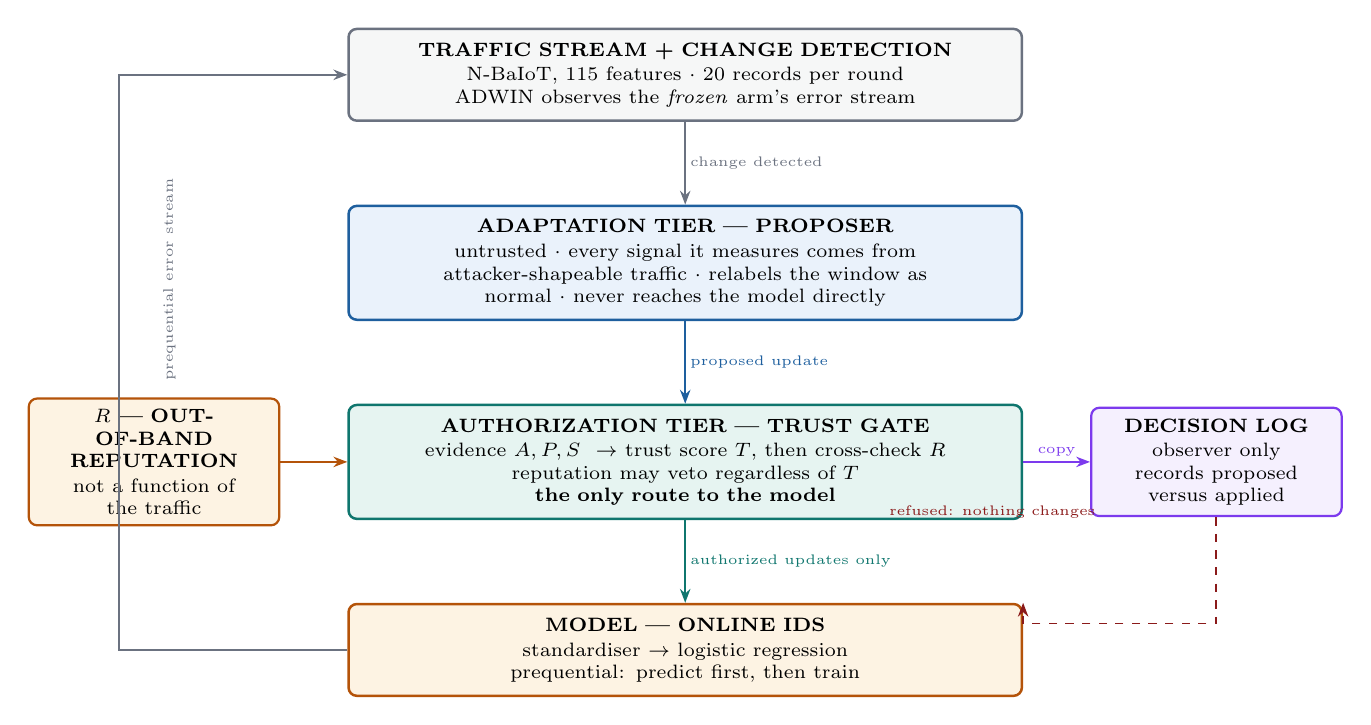
\begin{tikzpicture}[font=\scriptsize,node distance=0pt,
  box/.style={rounded corners=3pt,draw,line width=0.9pt,align=center,
              inner sep=5pt,text width=8.2cm},
  side/.style={rounded corners=3pt,draw,line width=0.8pt,align=center,
               inner sep=4pt,text width=2.9cm},
  ar/.style={-{Stealth[length=5pt]},line width=0.8pt},
  lbl/.style={font=\tiny,inner sep=1.5pt}]

\node[box,draw=cGrey,fill=cGrey!6] (src)
  {\textbf{TRAFFIC STREAM + CHANGE DETECTION}\\[1pt]
   N-BaIoT, 115 features $\cdot$ 20 records per round\\
   ADWIN observes the \emph{frozen} arm's error stream};

\node[box,draw=cBlue,fill=cBlueF,below=1.05cm of src] (prop)
  {\textbf{ADAPTATION TIER --- PROPOSER}\\[1pt]
   untrusted $\cdot$ every signal it measures comes from\\
   attacker-shapeable traffic $\cdot$ relabels the window as\\
   normal $\cdot$ never reaches the model directly};

\node[box,draw=cTeal,fill=cTealF,below=1.05cm of prop] (gate)
  {\textbf{AUTHORIZATION TIER --- TRUST GATE}\\[1pt]
   evidence $A,P,S \rightarrow$ trust score $T$, then cross-check $R$\\
   reputation may veto regardless of $T$\\
   \textbf{the only route to the model}};

\node[box,draw=cAmber,fill=cAmberF,below=1.05cm of gate] (model)
  {\textbf{MODEL --- ONLINE IDS}\\[1pt]
   standardiser $\rightarrow$ logistic regression\\
   prequential: predict first, then train};

\node[side,draw=cAmber,fill=cAmberF,left=0.85cm of gate] (rep)
  {\textbf{$R$ --- OUT-OF-BAND\\REPUTATION}\\[1pt]
   not a function of\\the traffic};

\node[side,draw=cPurple,fill=cPurpleF,right=0.85cm of gate] (log)
  {\textbf{DECISION LOG}\\[1pt] observer only\\ records proposed\\ versus applied};

\draw[ar,cGrey] (src) -- node[lbl,right] {change detected} (prop);
\draw[ar,cBlue] (prop) -- node[lbl,right] {proposed update} (gate);
\draw[ar,cTeal] (gate) -- node[lbl,right] {authorized updates only} (model);
\draw[ar,cAmber] (rep) -- (gate);
\draw[ar,cPurple] (gate) -- node[lbl,above] {copy} (log);

\draw[ar,cGrey] (model.west) -- ++(-2.9,0) |- ($(src.west)+(0,0)$);
\node[lbl,rotate=90,cGrey] at (-6.55,-2.6) {prequential error stream};

\draw[cRed,dashed,line width=0.7pt,-{Stealth[length=5pt]}]
  (log.south) -- ++(0,-1.35) -| (model.north east);
\node[lbl,cRed] at (3.9,-5.55) {refused: nothing changes};
\end{tikzpicture}
\caption{System architecture -- the single authorized route to the model. The
reputation channel enters from outside the traffic path; the decision log
returns nothing and cannot influence the model.}
\label{fig:arch}
\end{figure}

\section{Design}

\subsection{Data Flow Diagram}

Data flow in one round proceeds as follows. The stream source supplies twenty
records, each carrying a feature vector, a ground-truth label and metadata. Each
record is scored prequentially by all four arms, producing predictions and an
error signal; the frozen arm's error signal drives the change detector. If no
change window is open the round ends and nothing is learned. If a window is
open, the window is transformed into the calibrated feature space and the three
evidence signals are computed; the gate combines them with the reputation and
emits a decision. An accepted decision applies the update to that arm's model
and advances its trusted baseline and reference direction; a refused decision
alters nothing. Every decision, with its reason, flows to the log store, which
feeds both the offline analysis and the interactive replay.
Figure~\ref{fig:dfd} shows the arrangement.

\begin{figure}[htbp]
\centering
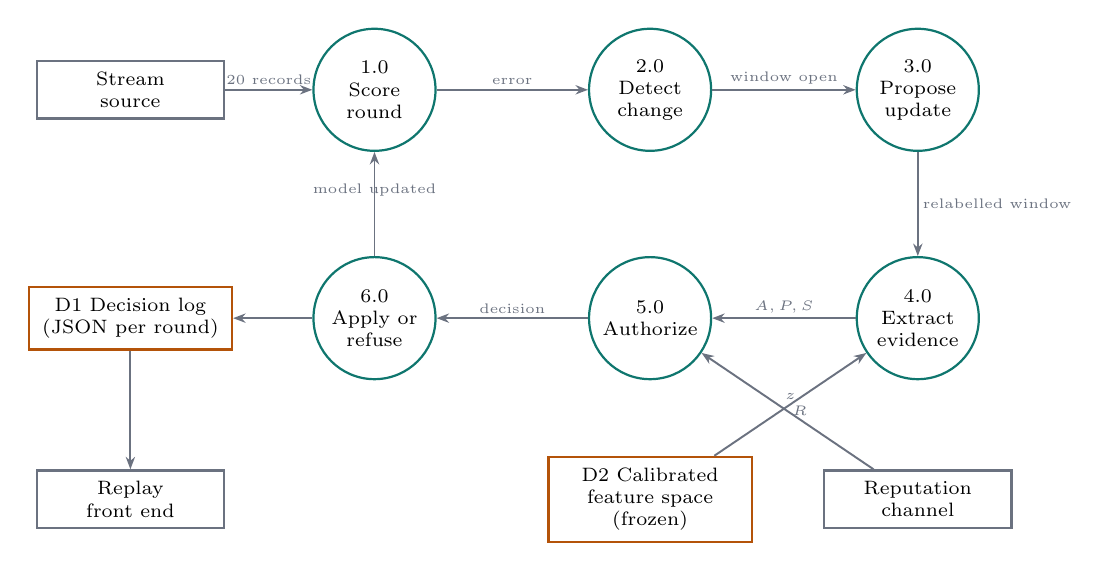
\begin{tikzpicture}[font=\scriptsize,
  proc/.style={circle,draw=cTeal,line width=0.8pt,align=center,
               inner sep=1pt,minimum size=1.55cm},
  store/.style={draw=cAmber,line width=0.8pt,align=center,inner sep=4pt,
                text width=2.3cm},
  ext/.style={draw=cGrey,line width=0.8pt,align=center,inner sep=4pt,
              text width=2.1cm},
  ar/.style={-{Stealth[length=4.5pt]},line width=0.7pt,cGrey},
  lbl/.style={font=\tiny,inner sep=1.5pt}]

\node[ext] (src) at (0,0) {Stream\\source};
\node[proc] (p1) at (3.1,0) {1.0\\Score\\round};
\node[proc] (p2) at (6.6,0) {2.0\\Detect\\change};
\node[proc] (p3) at (10.0,0) {3.0\\Propose\\update};
\node[proc] (p4) at (10.0,-2.9) {4.0\\Extract\\evidence};
\node[proc] (p5) at (6.6,-2.9) {5.0\\Authorize};
\node[proc] (p6) at (3.1,-2.9) {6.0\\Apply or\\refuse};
\node[store] (d1) at (0,-2.9) {D1 Decision log\\(JSON per round)};
\node[ext]  (op) at (0,-5.2) {Replay\\front end};
\node[store] (d2) at (6.6,-5.2) {D2 Calibrated\\feature space (frozen)};
\node[ext]  (rep) at (10.0,-5.2) {Reputation\\channel};

\draw[ar] (src) -- node[lbl,above] {20 records} (p1);
\draw[ar] (p1) -- node[lbl,above] {error} (p2);
\draw[ar] (p2) -- node[lbl,above] {window open} (p3);
\draw[ar] (p3) -- node[lbl,right] {relabelled window} (p4);
\draw[ar] (p4) -- node[lbl,above] {$A,P,S$} (p5);
\draw[ar] (rep) -- node[lbl,right] {$R$} (p5);
\draw[ar] (d2) -- node[lbl,above] {$z$} (p4);
\draw[ar] (p5) -- node[lbl,above] {decision} (p6);
\draw[ar] (p6) -- (d1);
\draw[ar] (d1) -- (op);
\draw[ar] (p6.north) -- ++(0,0.7) -| node[lbl,pos=0.25,above] {model updated} (p1.south);
\end{tikzpicture}
\caption{Data flow diagram (Level 1) -- one adaptation round.}
\label{fig:dfd}
\end{figure}

\subsection{Use Case Diagram}

The use cases in Figure~\ref{fig:uc} are derived from the implemented
interfaces -- the command-line entry points of the orchestrator and the controls
exposed by the replay front end -- rather than from a role model.

\note{Note on the actor model. The project defines no user roles, permissions or
authentication anywhere in its source. The single human actor is therefore named
for the interfaces it uses rather than derived from a documented role, and the
diagram should be read on that basis.}

\begin{figure}[htbp]
\centering
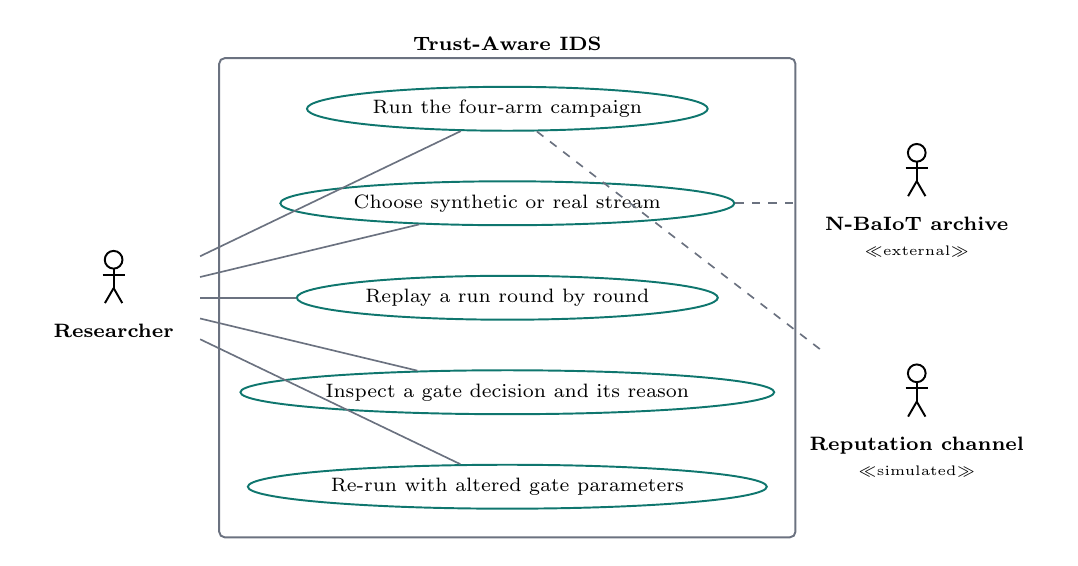
\begin{tikzpicture}[font=\scriptsize,
  uc/.style={draw=cTeal,line width=0.7pt,ellipse,align=center,
             inner sep=2.5pt,minimum width=3.5cm},
  ar/.style={line width=0.6pt,cGrey}]
\node (actor) at (0,-2.6) {\begin{tabular}{c}
  \tikz{\draw[line width=0.7pt] (0,0) circle (3.2pt);
        \draw[line width=0.7pt] (0,-0.11) -- (0,-0.36);
        \draw[line width=0.7pt] (-0.14,-0.19) -- (0.14,-0.19);
        \draw[line width=0.7pt] (0,-0.36) -- (-0.11,-0.55);
        \draw[line width=0.7pt] (0,-0.36) -- (0.11,-0.55);}\\[2pt]
  \textbf{Researcher}\end{tabular}};
\node[uc] (u1) at (5.0,-0.2) {Run the four-arm campaign};
\node[uc] (u2) at (5.0,-1.4) {Choose synthetic or real stream};
\node[uc] (u3) at (5.0,-2.6) {Replay a run round by round};
\node[uc] (u4) at (5.0,-3.8) {Inspect a gate decision and its reason};
\node[uc] (u5) at (5.0,-5.0) {Re-run with altered gate parameters};
\node (ext1) at (10.2,-1.4) {\begin{tabular}{c}
  \tikz{\draw[line width=0.7pt] (0,0) circle (3.2pt);
        \draw[line width=0.7pt] (0,-0.11) -- (0,-0.36);
        \draw[line width=0.7pt] (-0.14,-0.19) -- (0.14,-0.19);
        \draw[line width=0.7pt] (0,-0.36) -- (-0.11,-0.55);
        \draw[line width=0.7pt] (0,-0.36) -- (0.11,-0.55);}\\[2pt]
  \textbf{N-BaIoT archive}\\[-1pt]{\tiny$\ll$external$\gg$}\end{tabular}};
\node (ext2) at (10.2,-4.2) {\begin{tabular}{c}
  \tikz{\draw[line width=0.7pt] (0,0) circle (3.2pt);
        \draw[line width=0.7pt] (0,-0.11) -- (0,-0.36);
        \draw[line width=0.7pt] (-0.14,-0.19) -- (0.14,-0.19);
        \draw[line width=0.7pt] (0,-0.36) -- (-0.11,-0.55);
        \draw[line width=0.7pt] (0,-0.36) -- (0.11,-0.55);}\\[2pt]
  \textbf{Reputation channel}\\[-1pt]{\tiny$\ll$simulated$\gg$}\end{tabular}};
\foreach \u in {u1,u2,u3,u4,u5} \draw[ar] (actor) -- (\u);
\draw[ar,dashed] (u2) -- (ext1);
\draw[ar,dashed] (u1) -- (ext2);
\begin{scope}[on background layer]
\node[draw=cGrey,line width=0.7pt,rounded corners=2pt,
      fit=(u1)(u5),inner sep=10pt,label={[font=\scriptsize\bfseries,
      yshift=-1pt]above:Trust-Aware IDS}] {};
\end{scope}
\end{tikzpicture}
\caption{Use case diagram -- derived from the implemented interfaces.}
\label{fig:uc}
\end{figure}

\subsection{Class Diagram}

The principal classes are as follows. \texttt{OnlineIDS}
(\texttt{models/online\_ids.py}) wraps the River pipeline and owns the change
detector, exposing \texttt{score\_one} for prequential scoring and
\texttt{learn\_batch} for an authorized update. \texttt{FeatureSpace}
(\texttt{evidence/featurespace.py}) is the calibration-fitted, thereafter frozen
transform; it exposes \texttt{fit} and \texttt{transform} and deliberately
provides no method to refit. \texttt{TrustGate}
(\texttt{gate/trust\_gate.py}) holds the weights and thresholds and returns an
immutable \texttt{GateDecision} record carrying the authorization flag, the
three evidence values, the trust score, the reputation and a human-readable
reason. The evidence functions themselves are stateless. The orchestrator in
\texttt{experiments/run\_scenarios.py} owns the four \texttt{OnlineIDS}
instances, the two \texttt{TrustGate} instances and the per-gate mutable state
-- the trusted baseline $b$ and the reference direction $r$. This diagram is
marked optional in the report template and is described here rather than drawn.

\subsection{Sequence Diagram}

One round proceeds as follows. The orchestrator draws twenty records and asks
each of the four arms to predict and score every record, which updates the
prequential metrics and, for the frozen arm only, the change detector. The
orchestrator queries the change detector; if no window is open, it logs the
round and returns. Otherwise it constructs the proposed update by relabelling
every record in the window as normal, transforms the window into the calibrated
space, and for each gated arm computes the three evidence signals against
\emph{that arm's own} baseline and reference direction. Each gate returns a
decision. On acceptance the orchestrator applies the batch to that arm's model
and advances that arm's baseline and reference direction; on refusal it does
nothing at all. The ungated arm learns unconditionally and the frozen arm never
learns. Every arm's outcome is appended to the log. This diagram is marked
optional in the report template and is described here rather than drawn.

\section{Experimental Evaluation}

The mechanism is defined in Section~4.3.1, the experimental design in
Section~4.3.2, and the results in Sections~4.3.3 to 4.3.6.

\subsection{The Mechanism, and a Defect Found in It}

Evidence is computed in a feature space fitted on calibration benign records and
thereafter frozen:
\begin{equation}
z = \frac{\operatorname{sgn}(x)\odot\log(1+|x|)-\mu_{\mathrm{cal}}}
         {\sigma_{\mathrm{cal}}}.
\end{equation}
The three evidence signals are then, for a window with mean $\mu_w$, trusted
baseline $b$, previous window mean $\mu_{w-1}$ and reference direction $r$:
\begin{align}
\Delta_w &= \mu_w - b, &
A &= \operatorname{clip}\!\left(\tfrac{1}{2}\left(1+\tfrac{\Delta_w\cdot r}
     {\lVert\Delta_w\rVert\lVert r\rVert}\right),0,1\right),\\
P &= \frac{-\sum_i p_i\ln p_i}{\ln K},\ K=9, &
S &= \frac{1}{1+\lVert\mu_w-\mu_{w-1}\rVert}.
\end{align}
$A$ returns the neutral value $0.5$ while $r$ is undefined. The trust score and
the authorization rule are
\begin{equation}
T = 0.40A + 0.30P + 0.30S,\qquad
\mathrm{auth}=\begin{cases}
\textbf{false} & \text{if } R<\tau_R\quad(\text{veto})\\
\mathbb{1}[\,T\ge\tau_T\,] & \text{otherwise,}
\end{cases}
\end{equation}
with $\tau_T=0.55$ and $\tau_R=0.30$. On acceptance only,
$r \leftarrow 0.7r+0.3\Delta_w$ and $b \leftarrow \mu_w$.

\textbf{A defect found during integration.} The three signals are geometric:
they measure angles and norms between window mean vectors. That is only
meaningful if features contribute on comparable scales. On the synthetic stream
this held trivially. On real N-BaIoT it fails badly. Measured on the calibration
block, feature standard deviations span from $6.6\times10^{-3}$ to
$3.2\times10^{16}$, and individual feature maxima reach $5.67\times10^{17}$ --
roughly nineteen orders of magnitude.

Applying the evidence functions to raw vectors gives
$S = 1.7\times10^{-17}$, because $\lVert\Delta_w\rVert = 5.79\times10^{16}$. The
entire 0.30 weight on temporal stability is therefore dead in every round, for
every arm. Worse, five \texttt{HH\_jit\_*\_variance} columns account for
$71.8\%$, $11.6\%$, $6.6\%$, $5.4\%$ and $4.6\%$ of the shift vector's squared
norm -- together $100.0\%$ to one decimal place -- so a nominal ``cosine
similarity across 115 features'' is in reality a one-feature measurement.

The consequence is not subtle. A genuinely benign window scored $T = 0.5295$
against a threshold of $0.55$ and was \emph{refused}. With nothing ever
authorized, all four arms would have degenerated to the frozen arm and the
experiment would have shown nothing at all -- while still running to completion
and producing plausible-looking output. Table~\ref{tab:fix} records the same
window before and after the correction.

\begin{table}[htbp]
\centering
\caption{The same benign window, evaluated before and after the feature-space
correction. Raw-space geometry refuses legitimate traffic.}
\label{tab:fix}
\small
\begin{tabular}{@{}lccccc@{}}
\toprule
\textbf{Space} & $A$ & $P$ & $S$ & $T$ & \textbf{Decision}\\
\midrule
Raw features & 1.0000 & 0.4318 & $1.7\times10^{-17}$ & 0.5295 & refused\\
Signed-log, calibrated & 0.9097 & 0.8292 & 0.2572 & 0.6898 & authorized\\
\bottomrule
\end{tabular}
\end{table}

\note{This is reported because it is the kind of defect that does not announce
itself. The pipeline ran, produced numbers, and would have supported a confident
but empty conclusion. It was found by evaluating the evidence functions directly
on real windows rather than by inspecting end-to-end accuracy.}

\subsection{Experimental Design}

\textbf{Data.} Danmini\_Doorbell from N-BaIoT: \texttt{benign\_traffic.csv}
(49{,}548 records), \texttt{mirai\_attacks/scan.csv} (107{,}685) and
\texttt{gafgyt\_attacks/combo.csv} (59{,}718), each with 115 numeric features.
Integrity was checked before use: zero missing values, zero infinite values, and
identical column ordering across all three files. Twenty of the 115 columns take
negative values, which is why the transform is signed rather than absolute.
Ennio\_Doorbell benign traffic (39{,}100 records) provides a second benign
operating point.

\textbf{Arms.} Four detectors, identical apart from one property each: the
\emph{frozen} arm never updates; the \emph{ungated} arm accepts every proposal;
the \emph{traffic-only} gate applies $T\ge\tau_T$ with no veto; the
\emph{proposed} gate adds the reputation veto. All four share one change
trigger, driven by the frozen arm.

\textbf{Protocol.} 400 calibration records, then 80 rounds of 20 records,
prequential throughout. A change point opens a 15-round adaptation window.

\textbf{Scenario 2, slow poisoning.} Four phases: normal traffic (rounds 1--20);
paced poisoning (21--50), in which real Mirai records are interpolated toward
real benign records in signed-log space; the attack fully inside the benign
region (51--70); and a full-strength repeat of the calibrated attack (71--80).
Reputation is $0.05$ throughout every attack phase and $1.0$ for benign traffic.

\note{Interpolation is performed in signed-log space and inverted back to raw
values. Linear interpolation in raw space is dominated by the $10^{17}$-scale
columns and degenerates into a sudden attack preceded by a long flat prefix,
which is not the threat model.}

\subsection{Result: Slow Poisoning on Real Traffic}

\begin{table}[htbp]
\centering
\caption{Slow poisoning, real N-BaIoT, 80 rounds. Repeat-attack detection is the
mean windowed accuracy over rounds 71--80.}
\label{tab:main}
\small
\begin{tabular}{@{}lcccc@{}}
\toprule
\textbf{Arm} & \textbf{Accuracy} & \textbf{F1} &
\textbf{Repeat-attack} & \textbf{Updates accepted}\\
\midrule
Never learns (frozen) & 0.5531 & 0.5757 & \textbf{1.000} & 0 / 80\\
Learns from everything & 0.4531 & 0.4262 & 0.200 & 24 / 80\\
Checks traffic only & 0.4531 & 0.4262 & \textbf{0.200} & 5 / 80\\
\textbf{Proposed (traffic + reputation)} & 0.5531 & 0.5757 & \textbf{1.000} & 0 / 80\\
\bottomrule
\end{tabular}
\end{table}

The traffic-only gate accepted five of the twenty-four proposals and was
thereby corrupted: its detection of the subsequent full-strength repeat attack
fell to $0.200$, identical to the arm that accepted everything. The proposed
gate refused all twenty-four and retained detection of $1.000$, identical to the
frozen arm. Figure~\ref{fig:acc} shows the trajectories.

\begin{figure}[htbp]
\centering
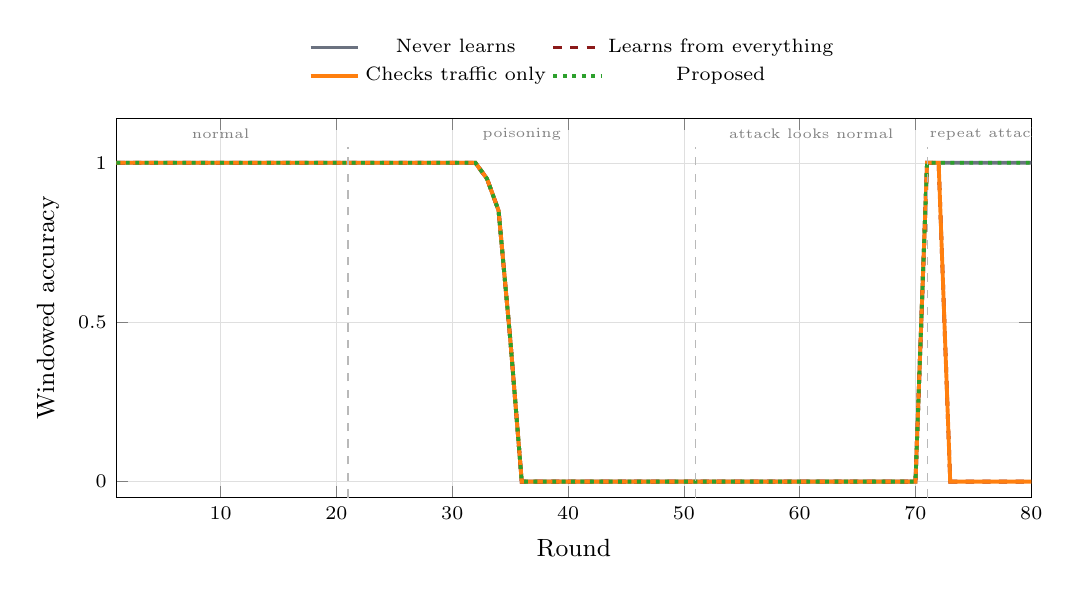
\begin{tikzpicture}
\begin{axis}[width=13.2cm,height=6.4cm,
  xlabel={Round},ylabel={Windowed accuracy},
  xmin=1,xmax=80,ymin=-0.05,ymax=1.14,
  legend style={at={(0.5,1.24)},anchor=north,legend columns=2,
                font=\scriptsize,draw=none},
  tick label style={font=\scriptsize},label style={font=\small},
  grid=major,grid style={line width=0.2pt,draw=gray!25}]
\addplot[cGrey,line width=1.4pt] coordinates {(1,1)(20,1)(32,1)(33,.95)(34,.85)(35,.45)(36,0)(70,0)(71,1)(80,1)};
\addlegendentry{Never learns}
\addplot[cRed,line width=1.4pt,dashed] coordinates {(1,1)(20,1)(32,1)(33,.95)(34,.85)(35,.45)(36,0)(70,0)(71,1)(72,1)(73,0)(80,0)};
\addlegendentry{Learns from everything}
\addplot[cOrange,line width=1.4pt] coordinates {(1,1)(20,1)(32,1)(33,.95)(34,.85)(35,.45)(36,0)(70,0)(71,1)(72,1)(73,0)(80,0)};
\addlegendentry{Checks traffic only}
\addplot[cGreen,line width=1.4pt,dotted] coordinates {(1,1)(20,1)(32,1)(33,.95)(34,.85)(35,.45)(36,0)(70,0)(71,1)(80,1)};
\addlegendentry{Proposed}
\draw[gray!55,dashed] (axis cs:21,-0.05) -- (axis cs:21,1.05);
\draw[gray!55,dashed] (axis cs:51,-0.05) -- (axis cs:51,1.05);
\draw[gray!55,dashed] (axis cs:71,-0.05) -- (axis cs:71,1.05);
\node[font=\tiny,gray] at (axis cs:10,1.09) {normal};
\node[font=\tiny,gray] at (axis cs:36,1.09) {poisoning};
\node[font=\tiny,gray] at (axis cs:61,1.09) {attack looks normal};
\node[font=\tiny,gray] at (axis cs:76,1.09) {repeat attack};
\end{axis}
\end{tikzpicture}
\caption{Windowed detection accuracy per round, real N-BaIoT. The frozen and
proposed arms coincide, as do the ungated and traffic-only arms. The divergence
at round 73 is the whole result.}
\label{fig:acc}
\end{figure}

\textbf{Why every arm scores zero from round 36 to round 70.} This is not a
failure of any arm. By round 36 the paced interpolation has carried the attack
traffic across the decision boundary, and in the third phase the attack records
are numerically identical to benign records -- verified to a maximum relative
difference of $4.7\times10^{-16}$ -- while still carrying an attack label. No
detector that inspects only traffic can score above zero there, including the
frozen arm, which never updated at all. This is why overall accuracy is a poor
headline for this experiment and repeat-attack detection is the meaningful
figure.

\subsection{Result: What Separated the Two Gates}

Table~\ref{tab:div} records every round on which the two gates disagreed.

\begin{table}[htbp]
\centering
\caption{The five rounds on which the traffic-only gate accepted an update the
proposed gate refused. At round 40 the evidence is numerically identical and
only $R$ separates the decisions.}
\label{tab:div}
\small
\begin{tabular}{@{}clccccll@{}}
\toprule
\textbf{Rd} & \textbf{Gate} & $A$ & $P$ & $S$ & $T$ & $R$ & \textbf{Decision}\\
\midrule
40 & traffic-only & 0.500 & 0.784 & 0.459 & 0.573 & 0.05 & accepted\\
40 & proposed     & 0.500 & 0.784 & 0.459 & 0.573 & 0.05 & \textbf{vetoed}\\
\midrule
72 & traffic-only & 0.956 & 0.480 & 0.509 & 0.679 & 0.05 & accepted\\
72 & proposed     & 0.500 & 0.480 & 0.509 & 0.497 & 0.05 & \textbf{vetoed}\\
73 & traffic-only & 0.753 & 0.480 & 0.555 & 0.612 & 0.05 & accepted\\
73 & proposed     & 0.500 & 0.480 & 0.555 & 0.510 & 0.05 & \textbf{vetoed}\\
74 & traffic-only & 0.770 & 0.306 & 0.633 & 0.590 & 0.05 & accepted\\
74 & proposed     & 0.500 & 0.306 & 0.633 & 0.482 & 0.05 & \textbf{vetoed}\\
75 & traffic-only & 0.777 & 0.306 & 0.633 & 0.593 & 0.05 & accepted\\
75 & proposed     & 0.500 & 0.306 & 0.633 & 0.482 & 0.05 & \textbf{vetoed}\\
\bottomrule
\end{tabular}
\end{table}

\textbf{Round 40 is the controlled comparison.} Both gates observed exactly the
same evidence, because neither had yet accepted anything and so both still held
the calibration baseline. $T = 0.573$ cleared the $0.55$ threshold. The
traffic-only gate accepted; the proposed gate refused on
$R = 0.05 < \tau_R = 0.30$. Nothing but the independent channel distinguishes
the two decisions.

\textbf{An unauthorized update is self-reinforcing.} From round 72 the two gates
no longer see the same evidence, and the reason is instructive. Having accepted
at round 40, the traffic-only gate advanced its own baseline $b$ and initialised
its reference direction $r$ -- using a poisoned window. Subsequent poisoned
windows then resembled that poisoned reference, so its attribution score rose
from the neutral $0.500$ to $0.956$, $0.753$, $0.770$ and $0.777$, carrying $T$
above threshold on each of the four rounds of the repeat attack. The proposed
gate's attribution remained pinned at exactly $0.500$ throughout the entire run,
because $r$ was never initialised: it never authorized anything.

Accepting one bad update therefore made the next one easier to accept. The
design decision that a refused update alters nothing -- not the model, not $b$,
not $r$ -- is what prevents that feedback loop, and it is why the proposed arm
finishes numerically identical to the frozen arm rather than merely better than
the ungated one.

\subsection{Result: Genuine Drift, a Negative Result}

Objective O7 asked for the complementary demonstration -- that the gate permits
legitimate adaptation. It was not achieved, and the reason is structural rather
than incidental.

Danmini's own benign file is stationary. The standardised distance between its
first and tenth decile blocks is $0.16$, while \emph{consecutive} blocks differ
by $0.30$ to $0.74$: the endpoints are closer together than neighbouring blocks
are. Splitting that file therefore yields no drift to detect. A second device,
Ennio\_Doorbell, provides a genuinely different benign operating point at a
distance of $5.7$ standard deviations in the calibrated space -- a shift some
thirty-six times larger.

Even so, no adaptation occurred. Table~\ref{tab:drift} records the outcome.

\begin{table}[htbp]
\centering
\caption{Genuine benign drift, real N-BaIoT, 70 rounds. No change point was
detected, so no update was proposed and all four arms are identical.}
\label{tab:drift}
\small
\begin{tabular}{@{}lcccc@{}}
\toprule
\textbf{Arm} & \textbf{Accuracy} & \textbf{Post-drift} &
\textbf{Updates accepted} & \textbf{Change windows}\\
\midrule
All four arms & 0.9979 & 0.993 & 0 / 70 & 0\\
\bottomrule
\end{tabular}
\end{table}

The explanation is that ADWIN observes an \emph{error} stream. A benign-to-benign
shift, however large in feature space, does not cross the decision boundary
between benign and Mirai traffic, so the frozen detector continued to classify
correctly at $0.998$ and produced no error signal to detect. Nothing degraded,
so nothing was proposed, so the gate was never asked to decide.

\note{Two readings of this are available and the report does not choose between
them. It may be argued that the behaviour is correct -- a detector that is still
working does not need to adapt. It may equally be argued that the trigger is
the wrong one, and that a distribution-based change detector operating on the
input rather than the error would have fired. Resolving this requires the
experiment the project did not run, and it is listed first under future work.}

\subsection{Cross-Check Against the Synthetic Stream}

The pipeline was also run on the synthetic generator used during development, as
a regression check that the real-data result is a property of the mechanism and
not of one dataset. Table~\ref{tab:synth} shows the same qualitative outcome:
the traffic-only gate is fooled and the proposed gate is not.

\begin{table}[htbp]
\centering
\caption{Slow poisoning on the synthetic stream. The pattern reproduces.}
\label{tab:synth}
\small
\begin{tabular}{@{}lcccc@{}}
\toprule
\textbf{Arm} & \textbf{Accuracy} & \textbf{F1} &
\textbf{Repeat-attack} & \textbf{Updates accepted}\\
\midrule
Never learns (frozen) & 0.6294 & 0.6718 & 1.000 & 0 / 80\\
Learns from everything & 0.5256 & 0.5375 & 0.200 & 37 / 80\\
Checks traffic only & 0.5256 & 0.5375 & 0.200 & 11 / 80\\
\textbf{Proposed} & 0.6294 & 0.6718 & 1.000 & 0 / 80\\
\bottomrule
\end{tabular}
\end{table}

On the synthetic stream the genuine-drift scenario \emph{does} exercise the
gate: the frozen arm falls to $0.000$ after the drift while the three adaptive
arms recover to $1.000$, and the proposed gate authorizes on 13 of 70 rounds --
exactly as many as the traffic-only gate, confirming that the veto does not
obstruct clean-reputation traffic. That this demonstration works on synthetic
data and not on real data is a limitation of the real scenario's construction,
as Section~4.3.5 describes, and not evidence that the veto over-refuses.

\subsection{Threats to Validity}

\textbf{The reputation channel is an oracle.} Keyed to ground-truth origin, it
never errs. A deployed feed would be stale, incomplete and occasionally wrong,
and the gate's behaviour under an unreliable $R$ is entirely unmeasured. This is
the single largest threat to the result's external validity.

\textbf{A single configuration.} One device, one attack family, one classifier,
one set of untuned thresholds, one poisoning schedule. No sensitivity analysis
was performed.

\textbf{Small denominators.} The headline figure rests on ten rounds of repeat
attack in a single run. No significance test is computed, and none would be
supportable.

\textbf{The threshold was not calibrated.} $\tau_T=0.55$ was chosen before any
real-data result was seen. Round 40 cleared it at $T=0.573$; a slightly higher
threshold would have refused that update and the traffic-only arm might have
survived. The result should be read as demonstrating a failure \emph{mode},
not as quantifying a failure \emph{rate}.

\textbf{No automated tests.} Specific claims were verified by direct
measurement, but the codebase has no regression suite, so silent breakage during
future modification is not guarded against.

% =====================================================================
\chapter{Conclusion and Future Work}

An authorization gate that consults a signal originating outside the traffic
channel refused a slow-poisoning campaign that defeated the equivalent gate
without that signal. On real N-BaIoT traffic the traffic-only gate accepted five
poisoned updates and afterwards detected an unmistakable repeat of the
calibrated attack only $20\%$ of the time; the proposed gate refused every
proposal and detected it every time. At the one round where both gates saw
numerically identical evidence, only the independent channel separated their
decisions.

Two findings beyond the headline are worth carrying forward. Traffic-derived
evidence is insufficient in principle rather than merely in practice, because
every component of it is measured from data the adversary is shaping; no
reweighting of $A$, $P$ and $S$ repairs that. And an unauthorized update is
self-reinforcing: accepting one poisoned window moved the traffic-only gate's
own frame of reference so that later poisoned windows scored \emph{better},
which is why the design principle that a refusal changes nothing at all matters
more than the specific thresholds.

Future work, in the order it should be attempted:

\begin{enumerate}[leftmargin=*,itemsep=3pt]
\item \textbf{A distribution-based change trigger} alongside the error-based
one, so that benign drift which does not degrade the detector still prompts a
review. This is what the genuine-drift scenario needs to become a demonstration
rather than a null result.
\item \textbf{A degraded reputation channel.} Measure the gate under a feed that
is stale, incomplete or wrong, which is the only way the present oracle result
becomes an engineering claim.
\item \textbf{An EWC or Fisher-freezing baseline}, to separate refusing a bad
update from resisting forgetting -- a distinction the current comparison asserts
but does not measure.
\item \textbf{Threshold and weight sensitivity}, converting a demonstrated
failure mode into a quantified failure rate.
\item \textbf{Breadth}: further devices, further attack families, and a
non-linear classifier.
\end{enumerate}

% =====================================================================
\chapter*{References}
\addcontentsline{toc}{chapter}{References}

\begin{list}{}{\leftmargin=1.2em\itemindent=-1.2em\itemsep=6pt}

\item [1] R. Sommer and V. Paxson, ``Outside the closed world: On using machine
learning for network intrusion detection,'' in \emph{Proc. IEEE Symp. Security
and Privacy}, Oakland, CA, USA, 2010, pp. 305--316.

\item [2] J. Gama, I. \v{Z}liobait\.{e}, A. Bifet, M. Pechenizkiy, and
A. Bouchachia, ``A survey on concept drift adaptation,'' \emph{ACM Computing
Surveys}, vol. 46, no. 4, art. 44, 2014.

\item [3] A. Bifet and R. Gavald\`a, ``Learning from time-changing data with
adaptive windowing,'' in \emph{Proc. SIAM Int. Conf. Data Mining}, Minneapolis,
MN, USA, 2007, pp. 443--448.

\item [4] J. Montiel, M. Halford, S. M. Mastelini, G. Bolmier, R. Sourty,
R. Vaysse, A. Zouitine, H. M. Gomes, J. Read, T. Abdessalem, and A. Bifet,
``River: Machine learning for streaming data in Python,'' \emph{Journal of
Machine Learning Research}, vol. 22, no. 110, pp. 1--8, 2021.

\item [5] Y. Meidan, M. Bohadana, Y. Mathov, Y. Mirsky, D. Breitenbacher,
A. Shabtai, and Y. Elovici, ``N-BaIoT---Network-based detection of IoT botnet
attacks using deep autoencoders,'' \emph{IEEE Pervasive Computing}, vol. 17,
no. 3, pp. 12--22, 2018.

\item [6] M. Barreno, B. Nelson, R. Sears, A. D. Joseph, and J. D. Tygar,
``Can machine learning be secure?,'' in \emph{Proc. ACM Symp. Information,
Computer and Communications Security}, Taipei, Taiwan, 2006, pp. 16--25.

\item [7] B. Nelson, M. Barreno, F. J. Chi, A. D. Joseph, B. I. P. Rubinstein,
U. Saini, C. Sutton, J. D. Tygar, and K. Xia, ``Exploiting machine learning to
subvert your spam filter,'' in \emph{Proc. USENIX Workshop on Large-Scale
Exploits and Emergent Threats}, San Francisco, CA, USA, 2008.

\item [8] B. Biggio, B. Nelson, and P. Laskov, ``Poisoning attacks against
support vector machines,'' in \emph{Proc. Int. Conf. Machine Learning},
Edinburgh, UK, 2012.

\item [9] M. Jagielski, A. Oprea, B. Biggio, C. Liu, C. Nita-Rotaru, and B. Li,
``Manipulating machine learning: Poisoning attacks and countermeasures for
regression learning,'' in \emph{Proc. IEEE Symp. Security and Privacy},
San Francisco, CA, USA, 2018, pp. 19--35.

\item [10] J. Kirkpatrick, R. Pascanu, N. Rabinowitz, J. Veness, G. Desjardins,
A. A. Rusu, K. Milan, J. Quan, T. Ramalho, A. Grabska-Barwi\'nska, D. Hassabis,
C. Clopath, D. Kumaran, and R. Hadsell, ``Overcoming catastrophic forgetting in
neural networks,'' \emph{Proc. National Academy of Sciences}, vol. 114, no. 13,
pp. 3521--3526, 2017.

\item [11] D. Arp, E. Quiring, F. Pendlebury, A. Warnecke, F. Pierazzi,
C. Wressnegger, L. Cavallaro, and K. Rieck, ``Dos and don'ts of machine learning
in computer security,'' in \emph{Proc. USENIX Security Symp.}, Boston, MA, USA,
2022.

\item [12] \emph{<<ExpIDS-style traffic-only gating reference -- insert from the
Review-1 literature table. This is the baseline the headline result is measured
against.>>}   %% TODO

\end{list}

\note{Verification status. Titles, authors, venues and years above are believed
correct. The page ranges on entries [1], [3], [6] and [9] are the fields most
likely to require correction and should be confirmed against the publisher
record before final submission.}

\end{document}
